\documentclass{beamer}
\usepackage{listings}
\usepackage[outdir=./images/]{epstopdf}
\definecolor{codegreen}{rgb}{0,0.6,0}
\definecolor{codegray}{rgb}{0.5,0.5,0.5}
\definecolor{codepurple}{rgb}{0.58,0,0.82}
\definecolor{backcolour}{rgb}{0.95,0.95,0.92}


\lstdefinestyle{mystyle}{
    backgroundcolor=\color{backcolour},
    commentstyle=\color{codegreen},
    keywordstyle=\color{magenta},
    numberstyle=\tiny\color{codegray},
    stringstyle=\color{codepurple},
    basicstyle=\ttfamily\footnotesize,
    breakatwhitespace=false,
    breaklines=true,
    captionpos=b,
    keepspaces=true,
    numbers=left,
    numbersep=5pt,
    showspaces=false,
    showstringspaces=false,
    showtabs=false,
    tabsize=2
}
\lstset{style=mystyle}


\usetheme{Frankfurt}
\beamertemplatenavigationsymbolsempty

\title{JaxFlowSim}

\author{Diego Renner}

\begin{document}

\section{Introduction}
\maketitle

\begin{frame}
	\frametitle{What}
	\begin{block}{What is jaxFlowSim?}
		\begin{itemize}
			\item 1D-haemodynamics solver
			\item written in JAX
			\item differentiable
		\end{itemize}
	\end{block}
	\vspace{5mm}
\end{frame}

\begin{frame}
	\frametitle{Why}
	\begin{block}{Motivation}
		\begin{itemize}
			\item towards personalised medicine
			\item parameter inference
			\item sensitivity analysis
		\end{itemize}
	\end{block}
	\vspace{5mm}
\end{frame}


\section{Code}

\begin{frame} [fragile]
	\frametitle{Code Structure}
	\begin{lstlisting}[basicstyle=\fontsize{8}{8}\selectfont\ttfamily, language=Python, caption=The code structure of an entire simulation is given here in pseudocode. Each line is detailed throughout this section., label=lst:pc, escapechar=|] 
		def runSimulation(config_filename, J) 
			config = loadConfig(config_filename) |\label{ln:init_start}|
			simulation_data = buildArterialNetwork(config) |\label{ln:init_end}|

			P_t = [0] |\label{ln:pt}|

			converged = False |\label{ln:whout1}|
			while not converged: |\label{ln:whout2}|
				t = 0 |\label{ln:t0}|
				i = 0 |\label{ln:i0}|
				P_t_temp = P_t |\label{ln:cp}|
				while t < T:
					dt = computeDt(simulation_data) |\label{ln:cfl}|
					simulation_data = setBoundaryValues(simulation_data, dt) |\label{ln:bv    }|
					simulation_data = muscl(simulation_data, dt) |\label{ln:muscl}|
					P_t[i,:] = savePressure(simulation_data) |\label{ln:svp}|
					t = t + dt |\label{ln:updt}|
					i = i + 1 |\label{ln:updi}|
					if i >= J:
						break
				converged = checkConv(P_t, P_t_temp) |\label{ln:conv}|
	\end{lstlisting}
\end{frame}
\begin{frame}
	\frametitle{Padding}
	without padding
	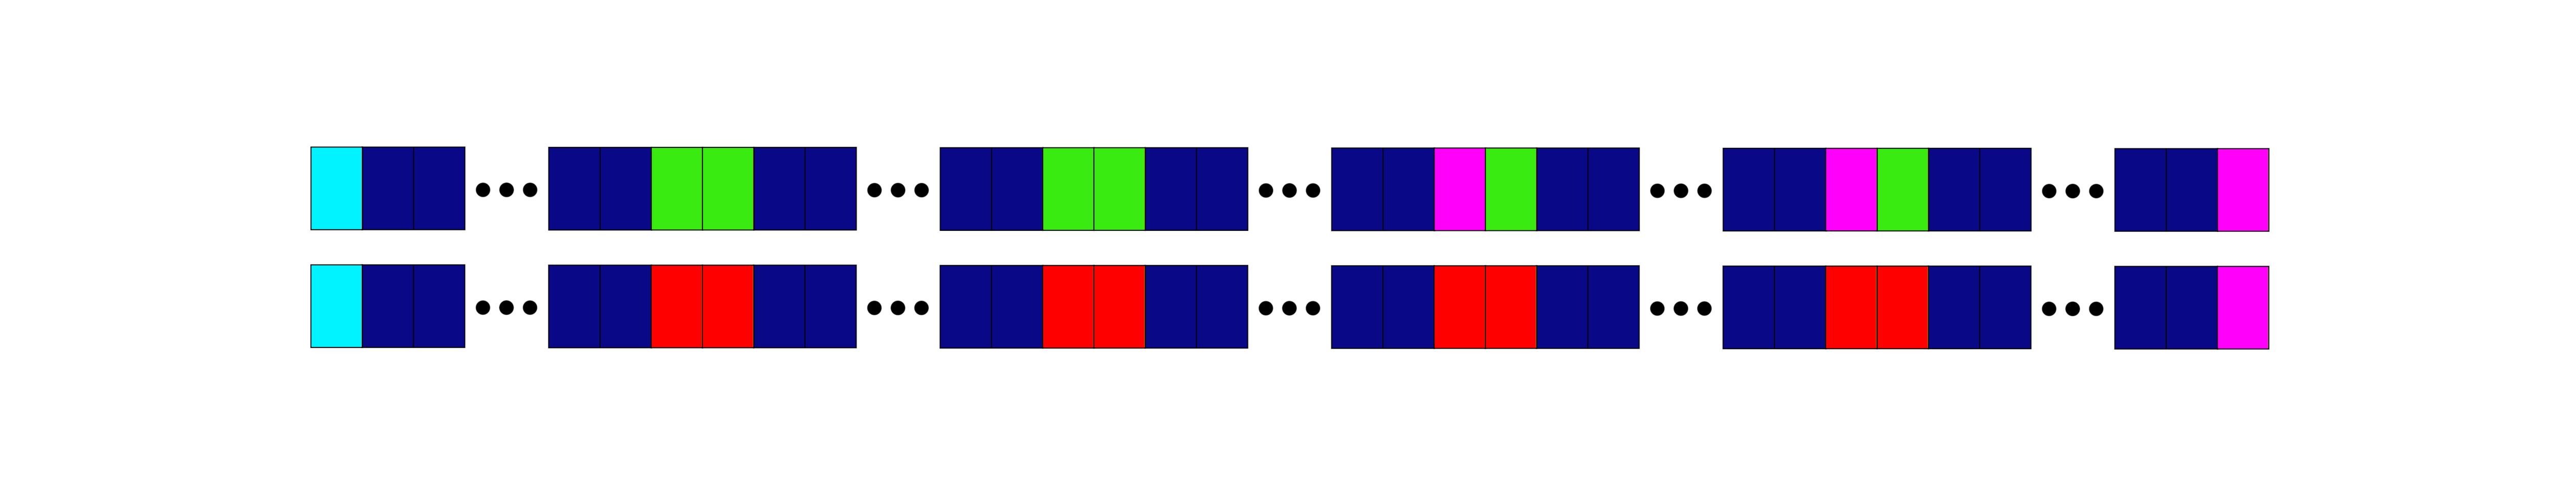
\includegraphics[width=\textwidth]{images/padding1.eps}
	with padding
	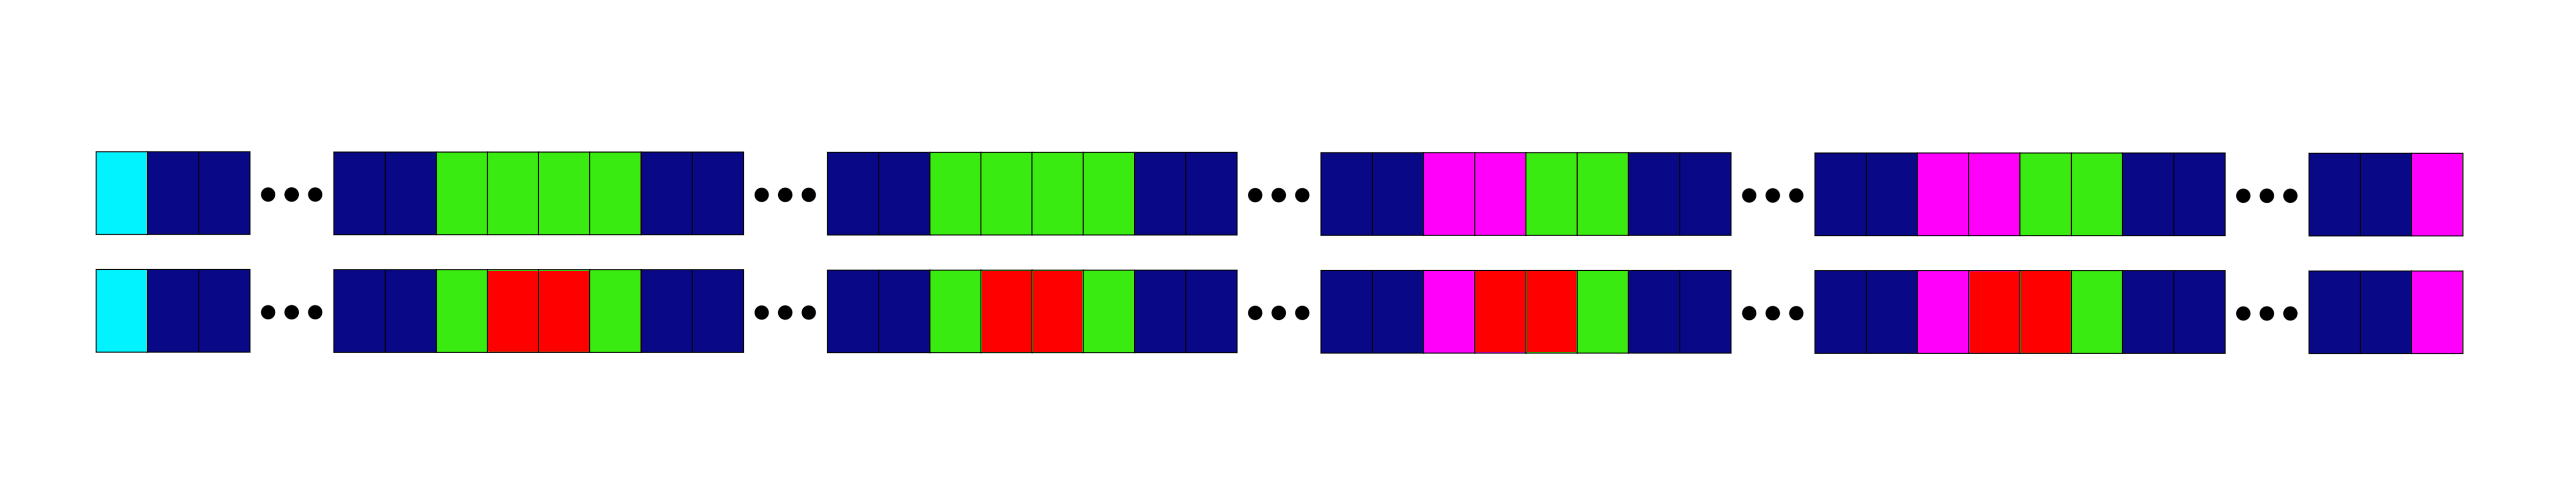
\includegraphics[width=\textwidth]{images/padding2.eps}
\end{frame}
	%    \frametitle{General Pipeline}
	%    \begin{enumerate}
	%        \item[1] Mesh $\longrightarrow$ 1x1 LEGO brick representation
	%        \item[2] Merge LEGO bricks greedily
	%        \item[3-4] Fix structural weakness
	%        \item[5] Print instructions 
	%    \end{enumerate}
	%    \vspace{5mm}
	%    \begin{columns}
	%        \column{0.2\textwidth}
	%            \includegraphics[height=0.265\textheight,width=\textwidth]{images/image-002.png}
	%            \begin{center}
	%                \color{blue} 1
	%            \end{center}
	%        \column{0.2\textwidth}
	%            \includegraphics[height=0.265\textheight,width=\textwidth]{images/image-001.png}
	%            \begin{center}
	%                \color{blue} 2
	%            \end{center}
	%        \column{0.2\textwidth}
	%            \includegraphics[height=0.265\textheight,width=\textwidth]{images/image-003.png}
	%            \begin{center}
	%                \color{blue} 3
	%            \end{center}
	%        \column{0.2\textwidth}
	%            \includegraphics[height=0.265\textheight,width=\textwidth]{images/image-004.png}
	%            \begin{center}
	%                \color{blue} 4
	%            \end{center}
	%        \column{0.2\textwidth}
	%            \includegraphics[height=0.265\textheight,width=\textwidth]{images/image-000.png}
	%            \begin{center}
	%                \color{blue} 5
	%            \end{center}
	%    \end{columns}
	%
%
%\begin{frame}
%    \frametitle{Merge Algorithm}
%    \begin{enumerate}
%        \item Choose brick at random.
%        \item Find the legal set of neighbors.
%        \item Select the neighbor with the lowest cost value and merge.
%        \item Goto step 2 until there are no more mergeable neighbors.
%        \item Goto step 1 until no brick can merge.
%    \end{enumerate}
%        \begin{figure}
%        \includegraphics[width=\textwidth]{images/image-005.png}
%        \caption{Possible legal set of neighbors.}
%        \end{figure}
%\end{frame}
%
%\begin{frame}
%    \frametitle{Merge Algorithm}
%    \begin{figure}
%    \begin{columns}
%        \column{0.4\textwidth}
%            \includegraphics[height=0.3\textheight, width=\textwidth]{images/image-010.png}
%            \includegraphics[height=0.3\textheight, width=\textwidth]{images/image-012.png}
%        \column{0.4\textwidth}
%            \includegraphics[height=0.3\textheight, width=\textwidth]{images/image-011.png}
%            \includegraphics[height=0.3\textheight, width=\textwidth]{images/image-013.png}
%    \end{columns}
%    \caption{Structure before and after merging (left), corresponding graph (right).}
%\end{figure}
%
%
%\end{frame}
%
%\begin{frame}
%    \frametitle{Solidity Optimization}
%    \begin{columns}
%        \column{0.5\textwidth}
%            \begin{enumerate}
%                \item Find bricks that connect two non-trivial subgraphs
%                \item Split these bricks and their neighbors
%                \item Merge again
%            \end{enumerate}
%        \column{0.5\textwidth}
%        \begin{figure}
%            \includegraphics[width=\textwidth]{images/image-014.png}
%            \caption{Points of structural weakness in graph representation.}
%        \end{figure}
%\end{columns}
%\end{frame}
%
%\begin{frame}
%    \frametitle{Extensions}
%    \begin{columns}
%        \column{0.5\textwidth}
%    \begin{itemize}
%        \item Pre-/Post-hollowing
%        \item Satisfying brick type limits 
%        \item Using colors
%    \end{itemize}
%    \column{0.5\textwidth}
%        \begin{figure}
%        \includegraphics[width=\textwidth]{images/image-017.png}
%        \caption{Hollowed layer for efficiency.}
%        \end{figure}
%
%    \end{columns}
%
%\end{frame}

\section{Demo}
%\begin{frame}
%    \frametitle{Setup and Results}
%    Setup: 
%    \begin{itemize}
%        \item Pre-hollowed as default
%        \item shell-size = 2
%        \item 1.8 GHz processor (sequential)
%        \item 20 trial runs, 5 models, 50 layer resolution
%    \end{itemize}
%    Results:
%    \begin{center}
%        \scalebox{0.5}{
%        \begin{tabular}{l l l l l l l l}
%            \hline \\ 
%            & & \multicolumn{2}{l}{no post-hollowing}  & \multicolumn{2}{l}{with post-hollowing} \\ \cline{3-4} \cline{5-6}& & \\
%            Mesh & Voxels & Time(sec) & Brick \# & Time(sec) & Brick \# &Conn Comp & Weak Pt \\
%            Eros & 15144 & 4.66 $\pm$ 1.35 & 3820 $\pm$ 25.5 & 5.51 $\pm$ 1.40 & 3110 $\pm$ 27.8 & 1 $\pm$ 0 & 0.100 $\pm$ 0.300 \\
%            Bunny & 11472 & 26.5 $\pm$ 5.98 & 2900 $\pm$ 21.4 & 27.0 $\pm$ 6.00 & 2380 $\pm$ 29.5 & 1 $\pm$ 0 & 7.20 $\pm$ 2.48 \\
%            Fertility & 6859 & 2.46 $\pm$ 1.21 & 1610 $\pm$ 17.9 & 2.78 $\pm$ 1.20 & 1400 $\pm$ 19.5 & 1 $\pm$ 0 & 0.050 $\pm$ 0.218 \\
%            Kitten & 12887 & 2.04 $\pm$ 0.728 & 3340 $\pm$ 28.4 & 2.72 $\pm$ 0.705 & 2650 $\pm$ 27.1 & 1 $\pm$ 0 & 0 $\pm$ 0 \\
%            Legoman & 9961 & 2.17 $\pm$ 0.846 & 2120 $\pm$ 24.9 & 2.50 $\pm$ 0.839 & 1800 $\pm$ 21.3 & 1 $\pm$ 0 & 0 $\pm$ 0 \\
%            \hline
%    \end{tabular}}
%    \end{center}
%\end{frame}
%
%\begin{frame}
%    \frametitle{Shortcomings and Future Work}
%    \begin{columns}
%        \column{0.5\textwidth}
%        \begin{figure}
%        \includegraphics[width=\textwidth]{images/image-018.png}
%        \caption{Example of a structure that can't be fully optimized.}
%        \end{figure}
%        \column{0.5\textwidth}
%        \begin{itemize}
%            \item Interactive visualization
%            \item Center of mass calculations
%            \item Parallelization
%        \end{itemize}
%    \end{columns}
%\end{frame}
%
%\begin{frame}
%    \frametitle{Conclusion}
%    \begin{columns}
%        \column{0.5\textwidth}
%    Compared to previous work:
%    \begin{itemize}
%        \item Faster \& more precise 
%        \item Solidity measure
%        \item Many extensions
%    \end{itemize}
%    \column{0.5\textwidth}
%        \begin{figure}
%        \includegraphics[width=\textwidth]{images/image-001.png}
%        \end{figure}
%
%\end{columns}
%\end{frame}    

\end{document}
